\section{Benchmark}
\label{sec:benchmark}

\subsection{Experimental Setup}
\label{sec:setup}

We test on two systems with different precision matrix structures.

\textbf{Lorenz~96.} The Lorenz~96 model~\cite{lorenz1996predictability} has $n = 40$ state variables with forcing $F = 8$, producing chaotic dynamics with dense off-diagonal precision structure due to spatial coupling. We use $m = 32$ randomly placed observations with Gaussian error $\sigma_o = 0.01$, multiplicative inflation $\rho = 1.05$, and 100 assimilation cycles at observation frequency $\Delta t_{\text{obs}} = 0.1$. Ensemble sizes are $N_e \in \{50, 60, 80, 100\}$, all above the $N_e > n + 2 = 42$ threshold required for direct precision methods. Each configuration is repeated 10 times with different random seeds.

\textbf{AR(1) cosmological model.} To test on data with near-diagonal precision structure, we build an AR(1) model calibrated to BOSS DR12 Patchy mock catalog statistics from Looijmans et al.~\cite{looijmans2024comparison}:
\begin{equation}
\label{eq:ar1}
\mathbf{x}_{t+1} = \phi \, \mathbf{x}_t + (1 - \phi) \, \boldsymbol{\mu} + \boldsymbol{\varepsilon}, \quad \boldsymbol{\varepsilon} \sim \mathcal{N}(\mathbf{0}, \mathbf{Q}),
\end{equation}
with $\boldsymbol{\mu}$ the mean power spectrum from the mocks, $\phi = 0.95$, and $\mathbf{Q} = (1 - \phi^2) \boldsymbol{\Sigma}_{\text{mock}}$ so the stationary distribution has covariance $\boldsymbol{\Sigma}_{\text{mock}}$. This preserves the near-diagonal precision structure within a dynamical system. We use $d = 18$ state variables (9 $k$-bins $\times$ 2 multipoles), $m = 14$ observations ($\approx 78\%$ coverage), $\sigma_o = 100$, inflation $\rho = 1.02$, and $N_e \in \{24, 30, 40, 50\}$.

We also replicate the standalone precision estimation experiment of Looijmans et al.\ using the same BOSS mock catalogs. For subsample sizes $n \in \{24, 30, 40, 50\}$, we draw $M = 100$ random subsets of $n$ mocks, compute each estimator's precision matrix, and measure the relative Frobenius loss against the true precision (computed from all 2048 mocks with Hartlap correction~\cite{hartlap2007your}):
\begin{equation}
\label{eq:matrix_loss}
\mathcal{L}(\hat{\boldsymbol{\Pi}}, \boldsymbol{\Pi}_{\text{true}}) = \frac{\|\hat{\boldsymbol{\Pi}} - \boldsymbol{\Pi}_{\text{true}}\|_F}{\|\boldsymbol{\Pi}_{\text{true}}\|_F}.
\end{equation}

Seven methods are compared on Lorenz~96: standard EnKF, EnKF-Cholesky (bandwidth $r = 2$), three direct precision shrinkage variants (identity, scaled identity, eigenvalue targets), NERCOME, and Ledoit-Wolf. The cosmological target is excluded from Lorenz~96 since this model does not produce power spectrum data; it is evaluated on the cosmological experiments alongside all other methods.

For filtering experiments, we report the relative RMSE of the analysis state:
\begin{equation}
\label{eq:rmse}
\text{RMSE}(t) = \frac{\|\bar{\mathbf{x}}^a(t) - \mathbf{x}^{\text{true}}(t)\|_2}{\|\mathbf{x}^{\text{true}}(t)\|_2},
\end{equation}
time-averaged over the last 50 cycles to discard the initial transient.

\subsection{Lorenz~96 Results}
\label{sec:lorenz_results}

Figure~\ref{fig:rmse_time} shows RMSE over 100 assimilation cycles for six methods at $N_e = 100$.

\begin{figure}[t]
\centering
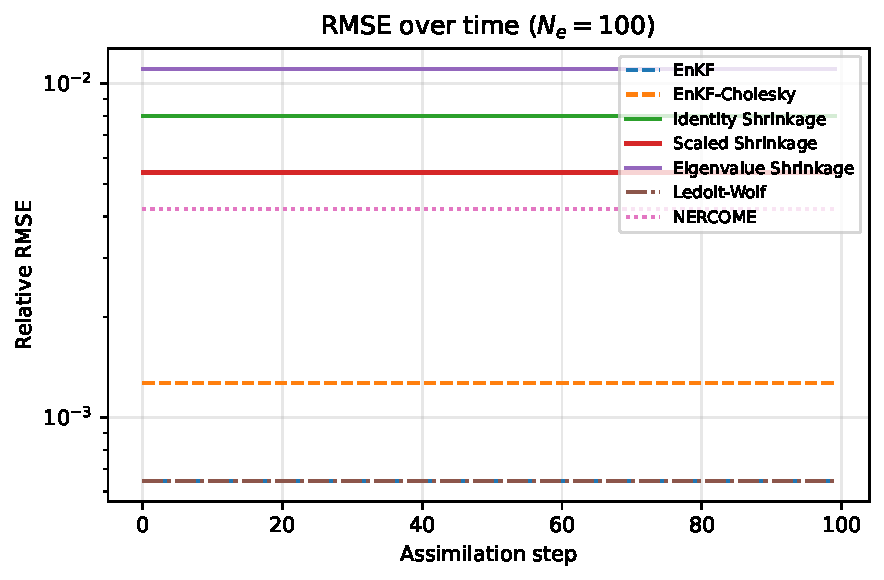
\includegraphics[width=0.9\textwidth]{figures/rmse_time.pdf}
\caption{Evolution of relative RMSE over 100 assimilation cycles for different analysis methods with $N_e = 100$. Shrinkage-based methods (solid lines) and Ledoit-Wolf (dash-dot) are compared against the standard EnKF and EnKF-Cholesky (dashed).}
\label{fig:rmse_time}
\end{figure}

Table~\ref{tab:performance} summarizes performance across ensemble sizes. Ledoit-Wolf achieves the lowest RMSE at three of four ensemble sizes, with near-zero variance across runs. The direct precision shrinkage methods show erratic non-monotonic behavior---RMSE sometimes jumps at intermediate ensemble sizes before dropping again---and high standard deviations reflecting seed-dependent instability.

\begin{table}[t]
\centering
\caption{Time-averaged relative RMSE ($\times 10^{-2}$) for different methods and ensemble sizes on Lorenz~96. Best result per column in \textbf{bold}. $^\dagger$Scaled Shrinkage is a novel domain-agnostic adaptation proposed in this work.}
\label{tab:performance}
\begin{tabular}{@{}lcccc@{}}
\toprule
Method & $N_e = 50$ & $N_e = 60$ & $N_e = 80$ & $N_e = 100$ \\
\midrule
EnKF (standard)          & $0.35 \pm 0.18$ & $0.38 \pm 0.56$ & $0.08 \pm 0.02$ & $\mathbf{0.06 \pm 0.01}$ \\
EnKF-Cholesky            & $0.14 \pm 0.01$ & $0.13 \pm 0.01$ & $0.13 \pm 0.01$ & $0.13 \pm 0.01$ \\
Identity Shrinkage       & $0.79 \pm 0.62$ & $1.53 \pm 1.62$ & $0.63 \pm 0.31$ & $0.81 \pm 0.82$ \\
Scaled Shrinkage$^\dagger$ & $0.43 \pm 0.20$ & $0.88 \pm 0.66$ & $0.51 \pm 0.24$ & $0.59 \pm 0.35$ \\
Eigenvalue Shrinkage     & $1.56 \pm 0.59$ & $2.00 \pm 2.11$  & $1.68 \pm 0.93$ & $1.30 \pm 1.25$ \\
NERCOME                  & $0.23 \pm 0.09$ & $0.29 \pm 0.18$  & $0.36 \pm 0.15$ & $0.42 \pm 0.19$ \\
Ledoit-Wolf              & $\mathbf{0.08 \pm 0.01}$ & $\mathbf{0.08 \pm 0.01}$ & $\mathbf{0.07 \pm 0.00}$ & $0.07 \pm 0.01$ \\
\bottomrule
\end{tabular}
\end{table}

This instability traces to the Bodnar coefficients. While $\alpha^*$ stays near $1 - n/N_e$ across all ensemble sizes and assimilation steps, $\beta^*$ is severely miscalibrated: unclamped values reach $10^8$--$10^9$ for the identity target and $10^3$--$10^5$ for the scaled target, requiring clamping to $[0,1]$ at every step. For the eigenvalue target, $\beta^*$ is effectively zero ($\sim 10^{-4}$), so no shrinkage toward the target occurs. The identity target $\boldsymbol{\Pi}_0 = \mathbf{I}$ is a poor match for Lorenz~96, whose precision matrix has significant off-diagonal entries from spatial coupling. In the formula for $\beta^*$~\eqref{eq:beta_star}, the $\text{tr}(\hat{\boldsymbol{\Pi}}_S \boldsymbol{\Pi}_0) / \|\boldsymbol{\Pi}_0\|_F^2$ factor becomes very large when the sample precision has large diagonal entries relative to the target norm, driving $\beta^*$ to extreme values. After clamping, the resulting precision matrices have condition numbers of $10^7$--$10^{11}$, making the analysis updates numerically unstable.

Figure~\ref{fig:rmse_vs_ne} plots the time-averaged RMSE against $N_e$. The standard EnKF and Ledoit-Wolf improve monotonically with larger ensembles. Modified Cholesky gives stable though not optimal performance across all sizes.

\begin{figure}[t]
\centering
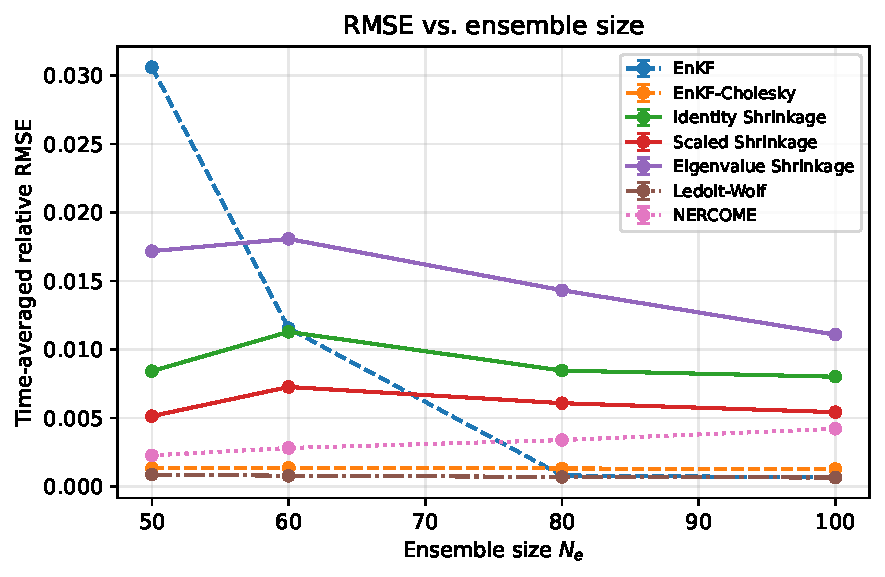
\includegraphics[width=0.9\textwidth]{figures/rmse_vs_ne.pdf}
\caption{Time-averaged relative RMSE (over last 50 cycles) as a function of ensemble size $N_e$ on Lorenz~96. Error bars show $\pm 1$ standard deviation over 10 runs.}
\label{fig:rmse_vs_ne}
\end{figure}

NERCOME shows a counterintuitive trend: RMSE \emph{increases} with ensemble size ($0.23$ at $N_e = 50$ to $0.42$ at $N_e = 100$). At small $N_e$, the sample covariance is noisy and bootstrap resampling provides genuine regularization; at larger $N_e$, the sample covariance is already reasonable, and bootstrap variance from 200 draws per cycle compounds over 100 sequential updates.

Figure~\ref{fig:precision_heatmap} compares the precision matrices produced by each method at a representative assimilation step.

\begin{figure}[t]
\centering
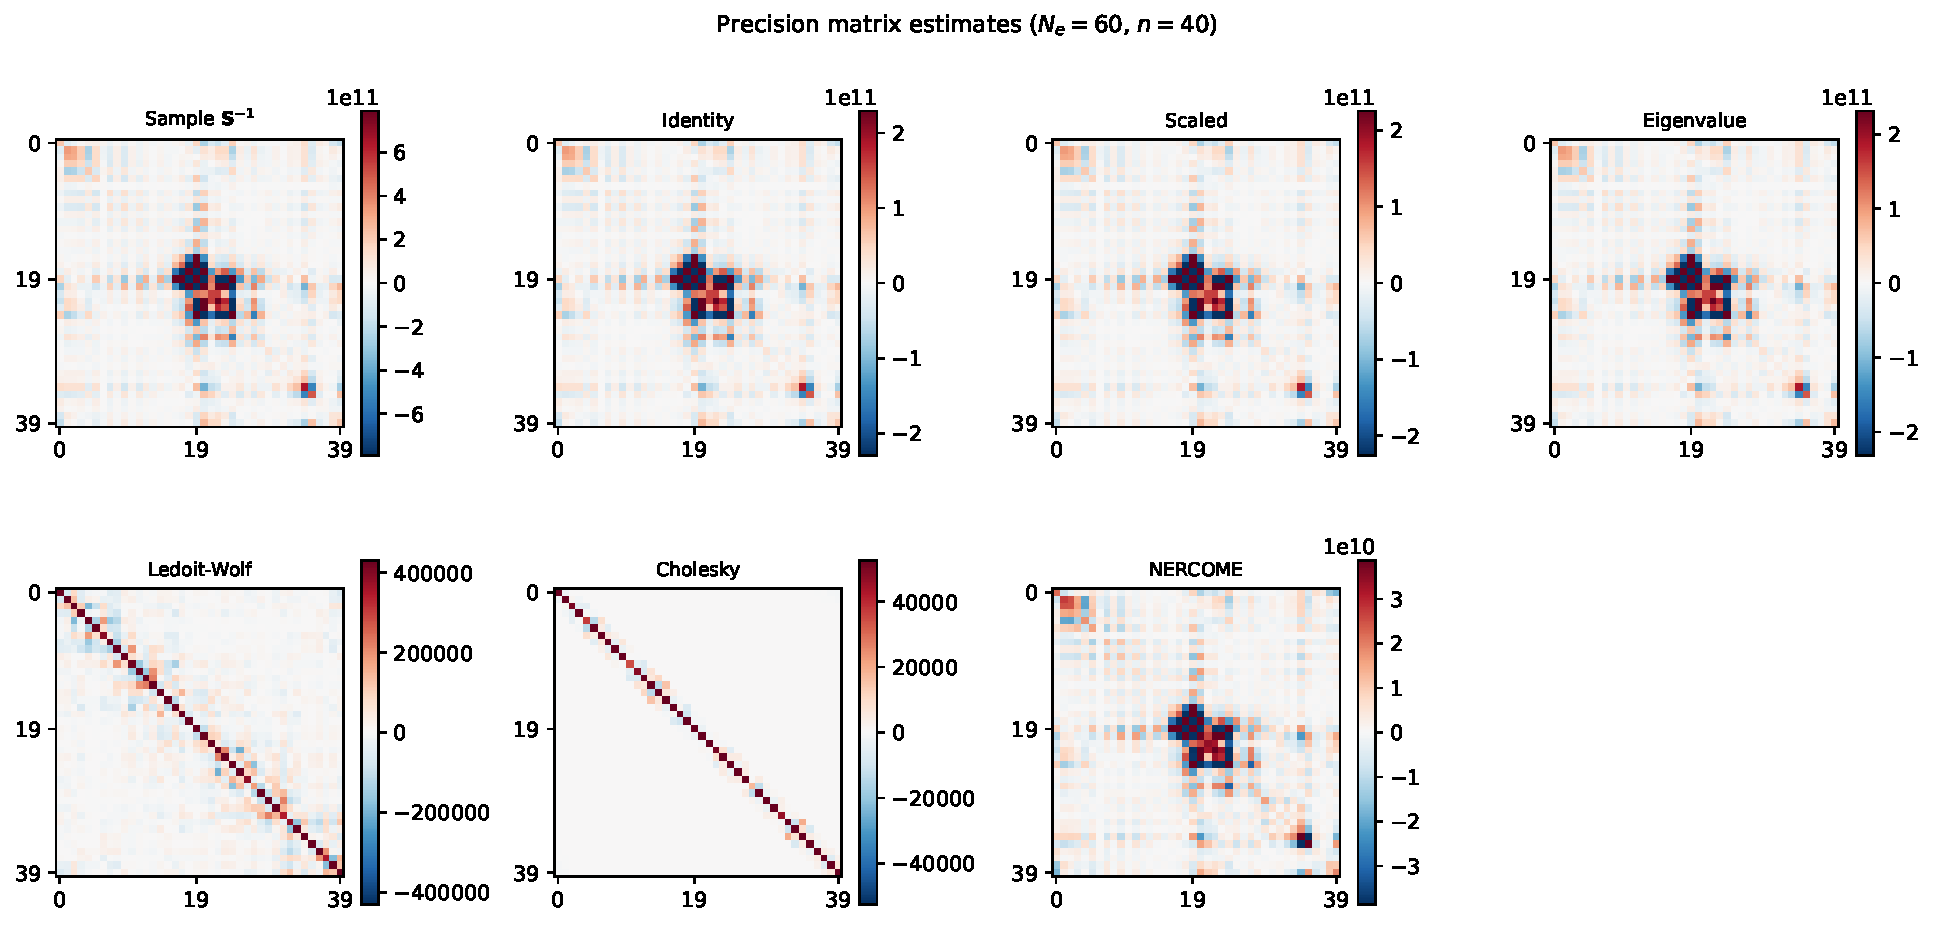
\includegraphics[width=0.9\textwidth]{figures/precision_heatmap.pdf}
\caption{Precision matrix estimates ($40 \times 40$) from different methods with $N_e = 60$: sample precision $\mathbf{S}^{-1}$, identity shrinkage, scaled shrinkage, eigenvalue shrinkage, Ledoit-Wolf, and modified Cholesky. The direct precision shrinkage estimators produce matrices with much larger magnitude than Ledoit-Wolf and Cholesky, reflecting the ill-conditioning discussed above.}
\label{fig:precision_heatmap}
\end{figure}

\subsection{Cosmological Results}
\label{sec:cosmo_results}

\subsubsection{Standalone Precision Estimation.}

Table~\ref{tab:cosmo_direct} shows the relative Frobenius loss for standalone precision matrix estimation on BOSS DR12 mock data. The results reverse compared to Lorenz~96: the direct precision shrinkage methods now outperform Ledoit-Wolf by a wide margin. At $n = 50$, the identity, eigenvalue, and cosmological targets all achieve losses of $\approx 0.41$ versus $0.93$ for Ledoit-Wolf. This confirms the findings of Looijmans et al.\ that direct precision shrinkage works well when the true precision matrix is near-diagonal.

\begin{table}[t]
\centering
\caption{Relative Frobenius loss of precision matrix estimates on BOSS DR12 mock data ($d = 18$). Lower is better. Best result per column in \textbf{bold}.}
\label{tab:cosmo_direct}
\begin{tabular}{@{}lcccc@{}}
\toprule
Method & $n = 24$ & $n = 30$ & $n = 40$ & $n = 50$ \\
\midrule
Sample (Hartlap)         & $1.15 \pm 1.01$ & $0.74 \pm 0.44$ & $0.47 \pm 0.15$ & $0.43 \pm 0.16$ \\
Identity Shrinkage       & $1.18 \pm 1.13$ & $0.68 \pm 0.43$ & $\mathbf{0.45 \pm 0.12}$ & $\mathbf{0.41 \pm 0.14}$ \\
Scaled Shrinkage$^\dagger$ & $0.90 \pm 0.96$ & $\mathbf{0.60 \pm 0.36}$ & $0.51 \pm 0.11$ & $0.46 \pm 0.13$ \\
Eigenvalue Shrinkage     & $1.20 \pm 1.13$ & $0.70 \pm 0.43$ & $0.46 \pm 0.13$ & $\mathbf{0.41 \pm 0.14}$ \\
Cosmological Shrinkage   & $1.19 \pm 1.13$ & $0.69 \pm 0.43$ & $0.46 \pm 0.13$ & $\mathbf{0.41 \pm 0.14}$ \\
NERCOME                  & $\mathbf{0.82 \pm 0.06}$ & $0.73 \pm 0.08$ & $0.63 \pm 0.08$ & $0.53 \pm 0.08$ \\
Ledoit-Wolf              & $0.96 \pm 0.01$ & $0.95 \pm 0.01$ & $0.94 \pm 0.01$ & $0.93 \pm 0.01$ \\
\bottomrule
\end{tabular}
\end{table}

Figure~\ref{fig:cosmo_matrix_loss} visualizes these trends. Ledoit-Wolf's loss stays nearly flat at $\approx 0.93$--$0.96$ regardless of subsample size: it shrinks the \emph{covariance} toward a diagonal target and then inverts, a suboptimal route when the precision matrix itself is near-diagonal. NERCOME does best at small $n$ thanks to its low variance, and the scaled identity target achieves the lowest mean loss at $n = 30$. Both are overtaken by the Bodnar methods once the sample size is large enough for the sample precision to become reliable.

\begin{figure}[t]
\centering
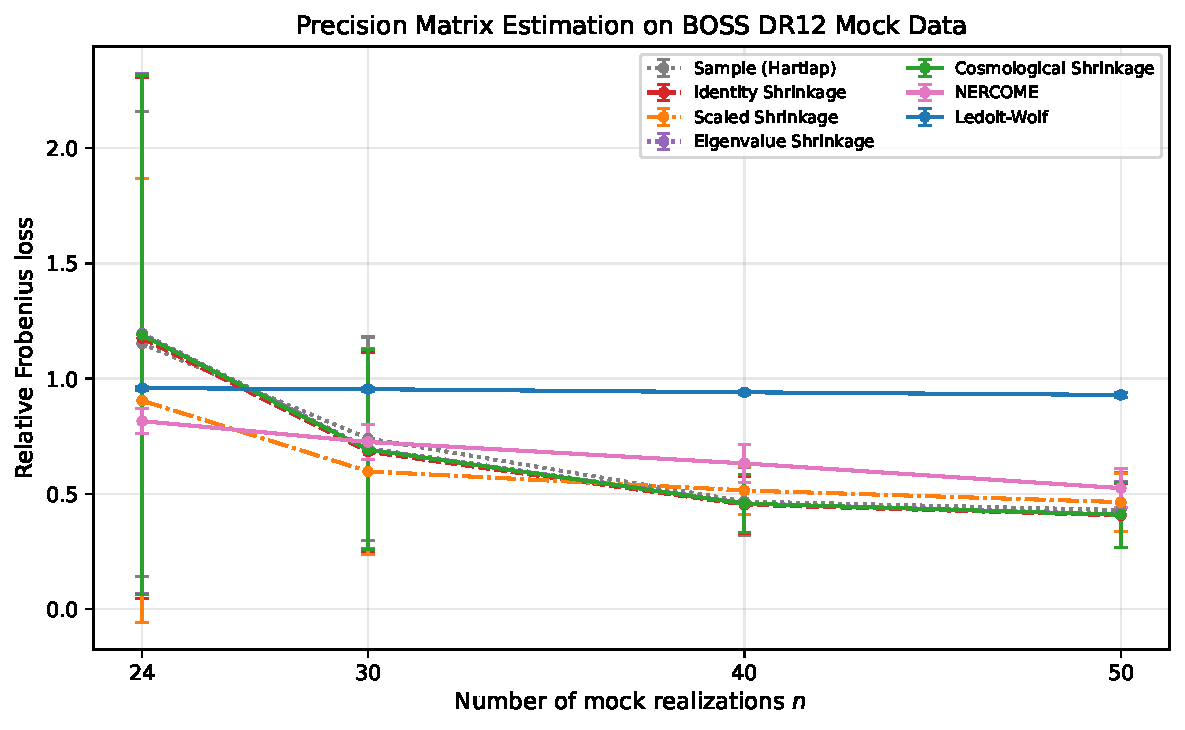
\includegraphics[width=0.9\textwidth]{figures/cosmo_matrix_loss.pdf}
\caption{Relative Frobenius loss of precision matrix estimates vs.\ subsample size on BOSS DR12 mock data ($d = 18$). Direct precision shrinkage methods (solid lines) achieve the lowest loss at $n \geq 40$, while Ledoit-Wolf (blue) remains flat near $0.93$. Error bars show $\pm 1$ standard deviation over 100 random draws.}
\label{fig:cosmo_matrix_loss}
\end{figure}

\subsubsection{EnKF Filtering.}

Table~\ref{tab:cosmo_enkf} reports the time-averaged RMSE for the AR(1) cosmological model. Ledoit-Wolf achieves the lowest RMSE at all four ensemble sizes, despite having the worst standalone precision estimates. Unlike on Lorenz~96, the direct precision shrinkage methods now improve smoothly and monotonically with ensemble size, confirming that the erratic Lorenz~96 behavior was caused by target-truth mismatch, not a fundamental flaw.

\begin{table}[t]
\centering
\caption{Time-averaged relative RMSE ($\times 10^{-2}$) for the AR(1) cosmological model. Best result per column in \textbf{bold}. $^\dagger$Scaled Shrinkage is a novel adaptation proposed in this work.}
\label{tab:cosmo_enkf}
\begin{tabular}{@{}lcccc@{}}
\toprule
Method & $N_e = 24$ & $N_e = 30$ & $N_e = 40$ & $N_e = 50$ \\
\midrule
EnKF (standard)          & $2.93 \pm 0.44$ & $2.20 \pm 0.34$ & $2.16 \pm 0.25$ & $2.06 \pm 0.39$ \\
EnKF-Cholesky            & $2.07 \pm 0.30$ & $1.76 \pm 0.20$ & $1.86 \pm 0.27$ & $1.86 \pm 0.37$ \\
Identity Shrinkage       & $2.03 \pm 0.27$ & $1.74 \pm 0.23$ & $1.86 \pm 0.21$ & $1.84 \pm 0.34$ \\
Scaled Shrinkage$^\dagger$ & $2.04 \pm 0.25$ & $1.73 \pm 0.20$ & $1.89 \pm 0.27$ & $1.85 \pm 0.33$ \\
Eigenvalue Shrinkage     & $2.39 \pm 0.28$ & $2.00 \pm 0.26$ & $2.01 \pm 0.23$ & $1.92 \pm 0.35$ \\
Cosmological Shrinkage   & $2.25 \pm 0.25$ & $2.00 \pm 0.28$ & $2.05 \pm 0.27$ & $1.97 \pm 0.36$ \\
NERCOME                  & $1.93 \pm 0.23$ & $1.79 \pm 0.21$ & $1.88 \pm 0.28$ & $1.90 \pm 0.33$ \\
Ledoit-Wolf              & $\mathbf{1.94 \pm 0.27}$ & $\mathbf{1.71 \pm 0.22}$ & $\mathbf{1.84 \pm 0.22}$ & $\mathbf{1.83 \pm 0.34}$ \\
\bottomrule
\end{tabular}
\end{table}

Figure~\ref{fig:cosmo_enkf_rmse} plots RMSE against ensemble size. All methods converge as $N_e$ grows. Pairwise Welch's $t$-tests ($n = 10$ runs) show that on Lorenz~96, Ledoit-Wolf's advantage is statistically significant ($p < 0.05$) at most ensemble sizes. On the cosmological data, most shrinkage methods do not differ significantly from Ledoit-Wolf ($p > 0.05$) at $N_e \geq 40$.

\begin{figure}[t]
\centering
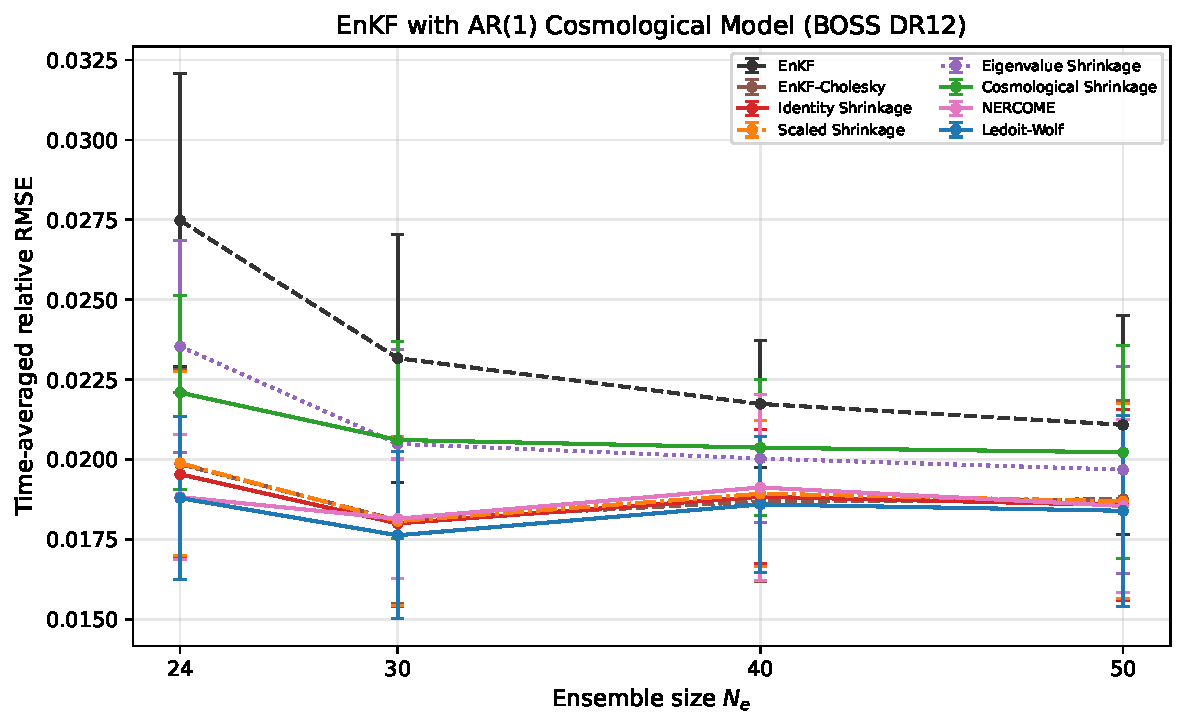
\includegraphics[width=0.9\textwidth]{figures/cosmo_enkf_rmse.pdf}
\caption{Time-averaged relative RMSE vs.\ ensemble size for the AR(1) cosmological model. All methods show stable, monotonic behavior---unlike the Lorenz~96 case (Figure~\ref{fig:rmse_vs_ne}). Ledoit-Wolf achieves the lowest RMSE throughout. Error bars show $\pm 1$ standard deviation over 10 runs.}
\label{fig:cosmo_enkf_rmse}
\end{figure}

The scaled identity target occupies a middle ground. On Lorenz~96, it outperforms the other direct precision variants (Table~\ref{tab:performance}), probably because scaling by empirical variances gives a better-conditioned target than the plain identity. On cosmological data, it achieves the lowest mean Frobenius loss at $n = 30$ (Table~\ref{tab:cosmo_direct}) but falls slightly behind the Bodnar methods at larger sample sizes. It serves its intended purpose: modest gains over the identity target without requiring external information, but no substitute for a domain-specific target when one is available.

\subsection{Estimation Quality vs.\ Filtering Performance}
\label{sec:estimation_vs_filtering}

The most striking result across both domains is the disconnect between standalone estimation quality and filtering performance. On cosmological data, the Bodnar et al.\ methods achieve Frobenius losses half those of Ledoit-Wolf (Table~\ref{tab:cosmo_direct}), yet Ledoit-Wolf yields the lowest EnKF RMSE (Table~\ref{tab:cosmo_enkf}).

The explanation is sequential accumulation. The precision estimator is applied at every assimilation cycle, and step-to-step variability compounds across 100 updates. Ledoit-Wolf's standard deviation across draws is $\pm 0.01$ in Part~A---an order of magnitude below the direct precision methods ($\pm 0.13$--$0.14$). A slightly biased but stable estimator beats a more accurate but variable one when errors accumulate over many cycles.

The dual-domain comparison confirms that the poor Lorenz~96 results for direct precision shrinkage reflect target-truth mismatch, not a deficiency of the methods. On Lorenz~96, diagonal targets produce erratic RMSE ($0.43$--$2.00 \times 10^{-2}$). On the near-diagonal cosmological data, the same methods achieve stable performance ($1.73$--$2.39 \times 10^{-2}$). The Bodnar framework works as designed when the target captures the dominant structure of the true precision matrix.

For sequential data assimilation, variance reduction matters at least as much as bias reduction.
